\section{Signal Model}
\label{sec:signal}

\begin{figure}[!htp]
\centering
    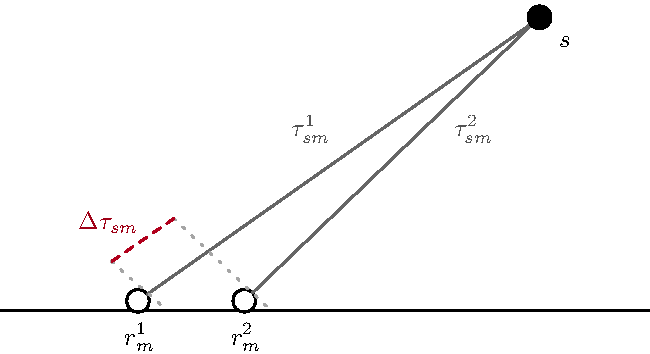
\includegraphics[scale=0.7]{data/figures/signal2}
    \caption{Direct propagation path for source $s$ and receiver pair $m$}
    \label{fig:signal}
\end{figure}

The basic configuration, as depicted in Figure \ref{fig:signal}, consists of two microphones that constitutes one sensor node. The received signal $x^i_m$ at microphone $i$ of pair $m$ can be described as a linear combination of the transfer function $a^i_{sm}$, multiplied bin-wise with the source signal $v_s$, and additive, spatially white noise $n^i_m$ in the \acrfull{stft} domain
\begin{equation}
	x_m^i(t,k)=\sum_{s=1}^{S}a_{sm}^i(t,k)\cdot v_s(t,k)+n_m^i(t,k).
	\label{eq:received_signal}
\end{equation}

%TODO: describe properties of noise

The direct path of the transfer function, that part corresponding to the line-of-sight, can be described as
\begin{equation}
	a_{sm}^i(t,k)\approx\frac{1}{\|\bm p_s-\bm p_m^i\|}\cdot\exp{\left(-j\frac{2\pi k}{K}\frac{\tau^i_{sm}}{T_s}\right)},
	\label{eq:acoustic_transfer_function}
\end{equation}

%TODO: transfer function <-> RIR

where $T_s$ is the sampling period of source signal $v_s$ and $\|\bm p_s-\bm p_m^i\|$ is the Eucledian distance between source position $\bm p_s$ and receiver position $\bm p^i_m$ of sensor node $m$. The signal travel time $\tau^i_{sm}$ between source position $\bm p_s$ and receiver position $\bm p^i_m$ is determined by the sound velocity $c$
\begin{equation}
	\tau^i_{sm}=\frac{\left(\|\bm p_s-\bm p_m^i\|\right)}{c}.
\end{equation}

To estimate the location of a source, we solve for the \gls{tdoa} $\Delta\tau_{sm}$, which we define as
\begin{equation}
    \Delta\tau_{sm}=\tau^2_{sm}-\tau^1_{sm}=\frac{\|\bm p_s-\bm p_m^2\|-\|\bm p_s-\bm p_m^1\|}{c},
\end{equation}

assuming planar wave fronts impinging on the microphones according to the far-field approximation of sound signals. From the \gls{tdoa}, the \gls{doa} can then be inferred with
\begin{equation}
    \text{DOA}=\arccos\left (\frac{c\cdot \Delta\tau_{sm}}{d_m}\right ),
\end{equation}
% TODO: Make the argument for TDOA, DOA and PRP bullet proof!

where $d_m$ is the Eucledian distance of the position of the two receivers $\bm p_m^1$ and $\bm p_m^2$ of sensor node $m$
\begin{equation}
    d_m=\| \bm p_m^1-\bm p_m^2\|.
\end{equation}

%TODO: Umformulieren des folgenden Absatz (RIR vs. Transfer function)
The direct path of the transfer function multiplied with the source signal contains the original phase information that is needed to estimate the position of the source. The remaining part of the received signal (the reverberant tail of the \gls{rir} multiplied with the source signal) distorts this information and will decrease the location estimation performance. 

%TODO: Klären, wann index s notwendig und wann nicht
Following \cite{Schwartz2014}, the \gls{prp} $\phi_{sm}(t,k)$ of the two signals $x_{sm}^1$ and $x_{sm}^2$ received at each sensor node $m$ will be used as the feature to be used for the purpose of localisation
\begin{equation}
    \phi_{sm}(t,k)=\frac{x^2_{sm}(t,k)}{x^1_{sm}(t,k)}\cdot \left |\frac{x^1_{sm}(t,k)}{x^2_{sm}(t,k)}\right |.
\label{eq:prp}
\end{equation}

To understand the link of \gls{prp} and \gls{doa}, let's solve the equation for two received signals\alt{ of equal volume (i.e. $|x^1(t,k)| = |x^2(t,k)|$)} in a noiseless environment (i.e., $n^i_{m}(t,k)=0$)
%\begin{equation}
%    \frac{x^2_{sm}}{x^1_{sm}}=\frac{v_{sm}\cdot a^2_{sm}}{v_{sm}\cdot a^1_{sm}}=\frac{\|\bm p_s-\bm p_m^1\|\cdot\exp{\left(-j\frac{2\pi k}{K}\frac{\tau^2_{sm}}{T_s}\right)}}{\|\bm p_s-\bm p_m^2\|\cdot\exp{\left(-j\frac{2\pi k}{K}\frac{\tau^1_{sm}}{T_s}\right)}}=\exp{\left ( j\frac{2\pi k}{K}\frac{(\tau^1-\tau^2)}{T_s}\right )}
%\end{equation}

\begin{equation}
    \phi_{sm}(t,k)=\exp{\left ( -j\frac{2\pi k}{K}\frac{\tau_{sm}^1-\tau_{sm}^2}{T_s}\right )}.
\end{equation}

As can be seen from the result, the amplitude has been eliminated by multiplication with $|x^1(t,k)|\ /\ |x^2(t,k)|$. The \gls{prp} feature can therefore be interpreted as the effect of the \gls{tdoa} on the phase difference between the two microphones of a sensor node.

%TODO: explain w-disjoint activity
The sources are assumed to exhibit w-disjoint orthogonality in the \gls{stft} domain \cite[p. 393]{Schwartz2014}, \cite{Rickard2006}.